\documentclass[a4paper,11pt,dvipsnames,addpoints]{exam}

\usepackage[english]{babel}
% Fonts %
\usepackage{fouriernc}
\usepackage[T1]{fontenc}

% Colors & Graphics %
\usepackage{xcolor}
\usepackage{graphicx}
\graphicspath{ {exam_figs/} }

% Tikz
\usepackage{tikz}
\usetikzlibrary{patterns}
\usepackage{tkz-euclide}

% Figures
\usepackage{float}
\usepackage{caption}
\usepackage{subcaption}

% Page Layout %
\usepackage[margin=1in]{geometry}

\pagestyle{headandfoot}
\firstpageheader{}{}{}
\runningfooter{}{}{}
\runningheader{Mock Exam}{Page~\thepage~of~\numpages}{\today}
\runningheadrule

% Math stuff %
\usepackage{amsmath}
\usepackage{amssymb}

% Fancy Headers %
\usepackage{enumitem}

% Tables %
\usepackage{booktabs}
\usepackage{tabularx}

\newcommand{\clr}{\textcolor{BrickRed}}
\newcommand{\clb}{\textcolor{RoyalBlue}}
\newcommand{\clg}{\textcolor{ForestGreen}}
\newcommand{\clf}{\textcolor{Fuchsia}}

% Rename solution
\setlength{\fboxsep}{8pt}

% Document %
\begin{document}
\marginpointname{~\%}
\bracketedpoints
\pointsinrightmargin

\begin{center}
 \Huge\sffamily Convex Polygons and Their Symmetries\\[4pt]
 \Large\sffamily 3.AB PreIB Maths -- Mock Exam
\end{center}

\begin{center}
\framebox{%
 \parbox{.7\textwidth}{%
  \centering
  Unless specified otherwise, you are to \textbf{\clr{always}} (at least
  briefly) explain your reasoning. Even in closed questions.
 }
}
\end{center}
\begin{questions}
 \question Definition of a polygon.
 \begin{parts}
  \part[10] Which of these shapes \emph{\clr{are not}} polygons?
  \textbf{Explain}.
  \begin{figure}[H]
   \centering
   \begin{subfigure}[b]{.2\textwidth}
    \centering
    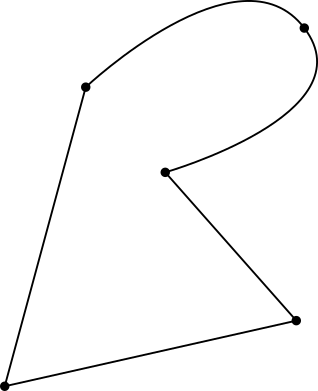
\includegraphics[width=\textwidth]{not_poly_1}
    \caption*{Option A.}
   \end{subfigure}
   \hfill
   \begin{subfigure}[b]{.2\textwidth}
    \centering
    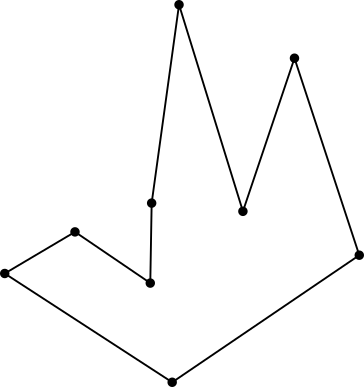
\includegraphics[width=\textwidth]{poly_1}
    \caption*{Option B.}
   \end{subfigure}
   \hfill
   \begin{subfigure}[b]{.2\textwidth}
    \centering
    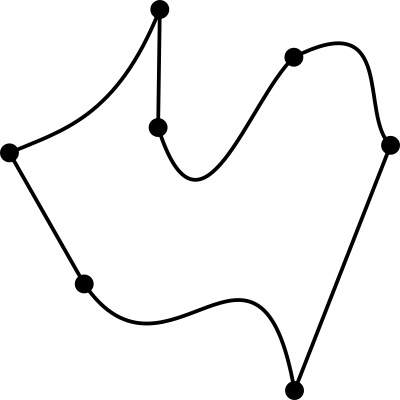
\includegraphics[width=\textwidth]{not_poly_2}
    \caption*{Option C.}
   \end{subfigure}
   \hfill
   \begin{subfigure}[b]{.2\textwidth}
    \centering
    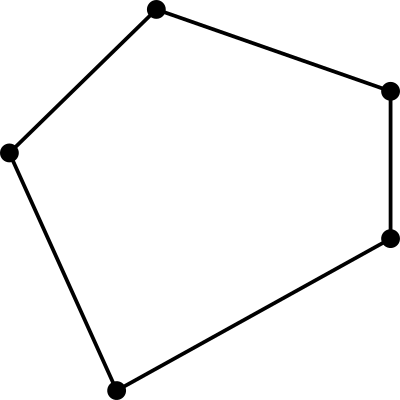
\includegraphics[width=\textwidth]{poly_2}
    \caption*{Option D.}
   \end{subfigure}
  \end{figure}
  \vspace{2in}
  \part[10] The sum of the sizes of all internal angles in a \emph{\clr{convex}}
  polygon on $n$ vertices is $(n-2) \cdot 180^{ \circ }$. How about
  \emph{\clb{non-convex}} polygons? Is there a number the sum of the sizes of
  internal angles in a non-convex polygon on $n$ vertices \textbf{cannot
  exceed}, or can it be infinite? Attempt to find such a number or construct a
  counterexample.
  \clearpage
 \end{parts}

 \question Triangulations of convex polygons.
 \begin{parts}
  \part[10] Draw all triangulations of the hexagon \emph{\clr{that can be
  reached in one flip}} from the one shown below. Use the provided shapes (not
  all of them necessarily). \textbf{No explanation required}.
  \begin{figure}[H]
   \centering
   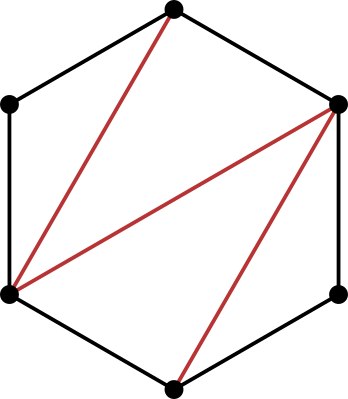
\includegraphics[width=.15\textwidth]{hexa_triangulation}

   \caption*{The initial triangulation.}
  \end{figure}
  \begin{figure}[H]
   \centering
   \begin{subfigure}[b]{.3\textwidth}
    \centering
    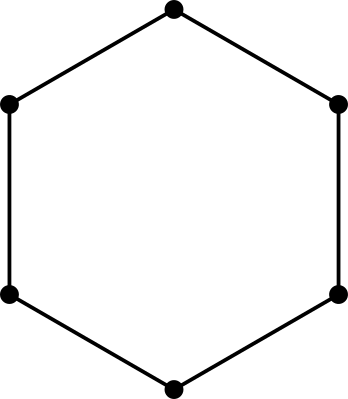
\includegraphics[width=.5\textwidth]{hexa_plain}
   \end{subfigure}
   \begin{subfigure}[b]{.3\textwidth}
    \centering
    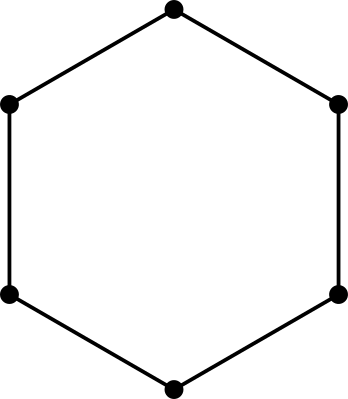
\includegraphics[width=.5\textwidth]{hexa_plain}
   \end{subfigure}
   \begin{subfigure}[b]{.3\textwidth}
    \centering
    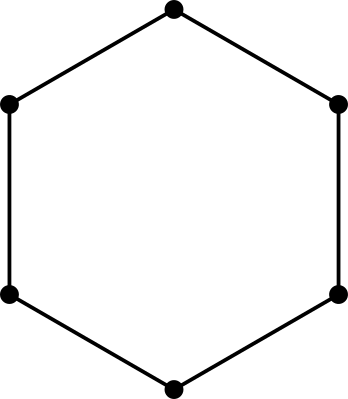
\includegraphics[width=.5\textwidth]{hexa_plain}
   \end{subfigure}
  \end{figure}
  \begin{figure}[H]
   \centering
   \begin{subfigure}[b]{.3\textwidth}
    \centering
    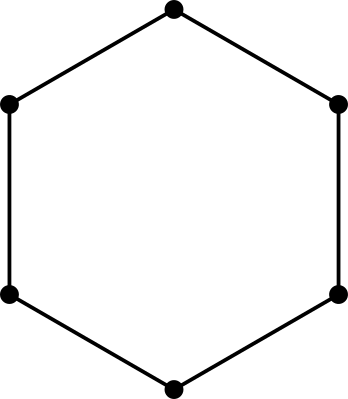
\includegraphics[width=.5\textwidth]{hexa_plain}
   \end{subfigure}
   \begin{subfigure}[b]{.3\textwidth}
    \centering
    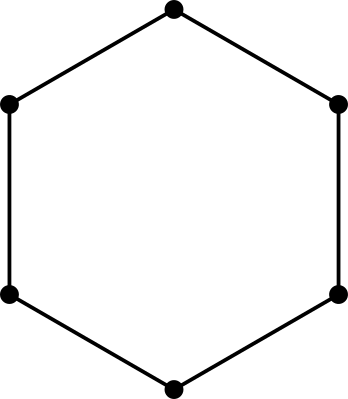
\includegraphics[width=.5\textwidth]{hexa_plain}
   \end{subfigure}
   \begin{subfigure}[b]{.3\textwidth}
    \centering
    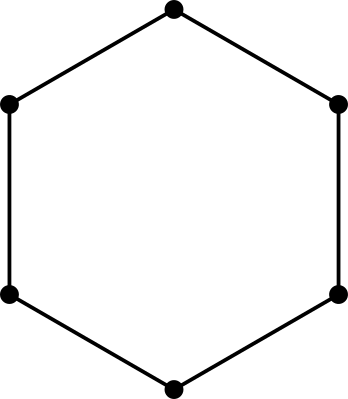
\includegraphics[width=.5\textwidth]{hexa_plain}
   \end{subfigure}
   \caption*{Shapes to draw diagonals into.}
  \end{figure}
  \part[10] The minimum number of flips to get from one triangulation of the
  hexagon to the \emph{\clr{same triangulation}} \textbf{without flipping the
  same diagonal twice in a row} is four. One such path is depicted below.
  \begin{center}
   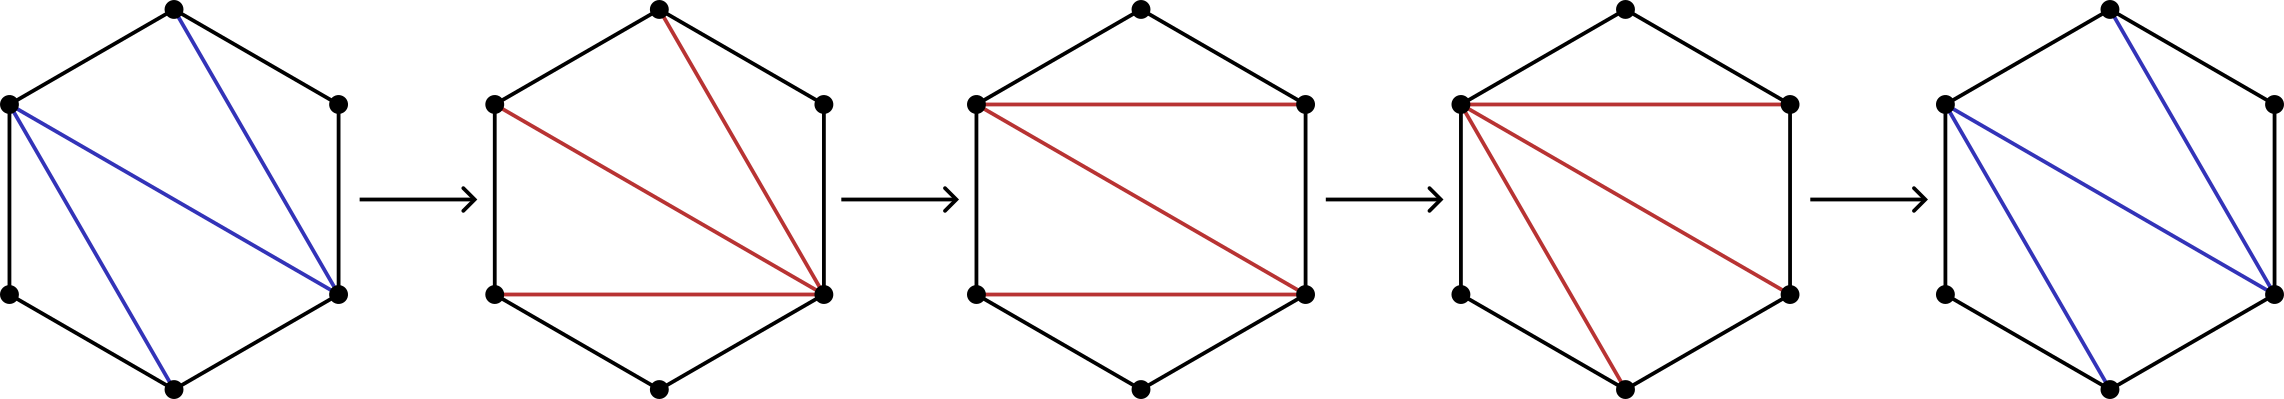
\includegraphics[width=.8\textwidth]{hexa_cycle}
  \end{center}
  Try to argue that \emph{\clr{there are only two paths}} of four flips, this
  one and its reverse. \emph{Notice that the `middle' diagonal remained stable}.
 \end{parts}
 \clearpage
 \question Plane transformations.
 \begin{parts}
  \part[10] Find out the \emph{\clr{image}} (the resulting shape when
  transformed) of a square (depicted below) under the plane transformation
  $\clb{f}(x,y) = (y,-x)$. \textbf{Provide a short explanation}.
  \begin{figure}[H]
   \centering
   \begin{subfigure}[c]{.3\textwidth}
    \centering
    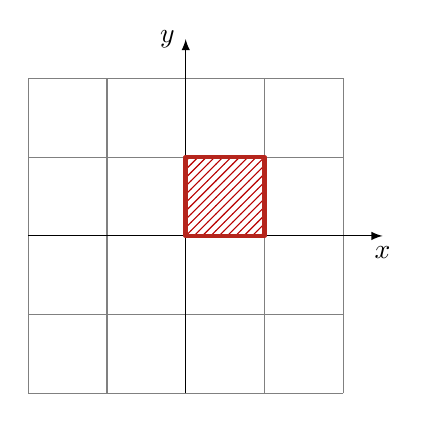
\begin{tikzpicture}
     \tkzInit[xmin=-2,xmax=2,ymin=-2,ymax=2]
     \tkzGrid
     \tkzDrawX
     \tkzDrawY
     \tkzDefPoints{0/0/a,0/1/b,1/1/c,1/0/d}
     \tkzDrawPolygon[ultra thick,BrickRed,pattern={north east lines}, pattern
     color=BrickRed](a,b,c,d)
    \end{tikzpicture}
    \caption*{The initial \clr{square}.}
   \end{subfigure}
   \hspace*{-2em}
   \begin{subfigure}[b]{.3\textwidth}
    \centering
    \begin{tikzpicture}
     \node (origin) at (0,0) {};
     \draw[-latex,thick,bend left=30,RoyalBlue] (0,1) to
      node[midway,yshift=3mm]{$f$} (4,1);
    \end{tikzpicture}
   \end{subfigure}
   \begin{subfigure}[c]{.3\textwidth}
    \centering
    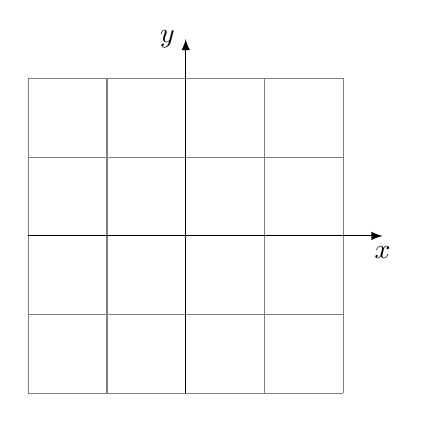
\begin{tikzpicture}
     \tkzInit[xmin=-2,xmax=2,ymin=-2,ymax=2]
     \tkzGrid
     \tkzDrawX
     \tkzDrawY
    \end{tikzpicture}
    \caption*{Draw the resulting shape here.}
   \end{subfigure}
  \end{figure}
  \vspace{2in}
  \part[10] Below, you see a unit square transformed by a plane transformation
  $\clg{g}$. Figure out \emph{one possible prescription} of this transformation,
  that is, write the coordinates of the point $\clg{g}(x,y)$ using $x$ and $y$.
  \begin{figure}[H]
   \centering
   \begin{subfigure}[c]{.3\textwidth}
    \centering
    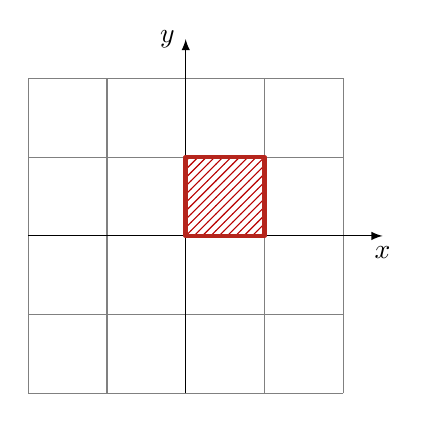
\begin{tikzpicture}
     \tkzInit[xmin=-2,xmax=2,ymin=-2,ymax=2]
     \tkzGrid
     \tkzDrawX
     \tkzDrawY
     \tkzDefPoints{0/0/a,0/1/b,1/1/c,1/0/d}
     \tkzDrawPolygon[ultra thick,BrickRed,pattern={north east lines}, pattern
     color=BrickRed](a,b,c,d)
    \end{tikzpicture}
    \caption*{The \clr{initial} square.}
   \end{subfigure}
   \hspace*{-2em}
   \begin{subfigure}[b]{.3\textwidth}
    \centering
    \begin{tikzpicture}
     \node (origin) at (0,0) {};
     \draw[-latex,thick,bend left=30,ForestGreen] (0,1) to
      node[midway,yshift=3mm]{$g$} (4,1);
    \end{tikzpicture}
   \end{subfigure}
   \begin{subfigure}[c]{.3\textwidth}
    \centering
    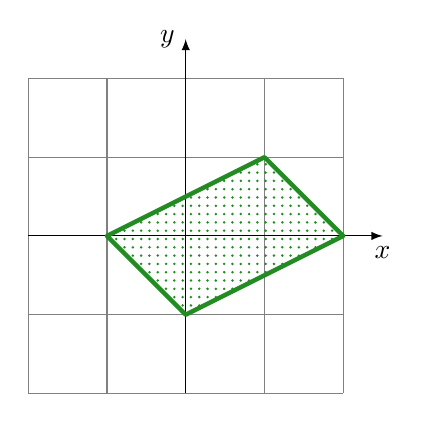
\begin{tikzpicture}
     \tkzInit[xmin=-2,xmax=2,ymin=-2,ymax=2]
     \tkzGrid
     \tkzDrawX
     \tkzDrawY
     \tkzDefPoints{0/-1/a,-1/0/b,1/1/c,2/0/d}
     \tkzDrawPolygon[ultra thick,ForestGreen,pattern={dots}, pattern
     color=ForestGreen](a,b,c,d)
    \end{tikzpicture}
   \caption*{The \clg{transformed} square.}
   \end{subfigure}
  \end{figure}
 \end{parts}
 \clearpage
 \question Symmetries of regular polygons.
 \begin{parts}
  \part[10] Given two symmetries of the \emph{square} -- the rotation $\clr{r} =
  ~\circlearrowleft 180^{ \circ }$ by $180^{ \circ }$ counter-clockwise and the
  reflection $\clb{s}$ drawn below -- determine (using any method you wish) the
  composition $\clr{r}\clb{s}$. \textbf{Explain}.
  \begin{center}
   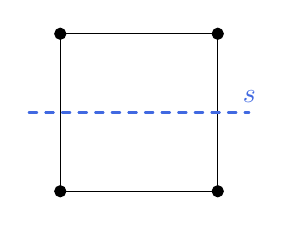
\begin{tikzpicture}[scale=2]
    \tkzInit
    \tkzDefPoints{0/0/a,0/1/b,1/1/c,1/0/d}
    \tkzDrawPoints[size=4,fill=black](a,b,c,d)
    \tkzDefMidPoint(a,b)\tkzGetPoint{m1}
    \tkzDefMidPoint(c,d)\tkzGetPoint{m2}
    \tkzDrawPolygon(a,b,c,d)
    \tkzDrawLine[thick,dashed,RoyalBlue](m1,m2)
    \tkzLabelLine[pos=1.2,yshift=2mm](m1,m2){$\clb{s}$}
   \end{tikzpicture}
  \end{center}
  \vspace{2in}
  \part[10] Given two symmetries of the hexakaidecagon (16 vertices) -- the
  reflections $\clr{s_1}$ and $\clb{s_2}$ depicted below -- compute (using any
  method you wish) the composition $\clr{s_1}\clb{s_2}$. \textbf{Explain}.
  \begin{figure}[H]
   \centering
   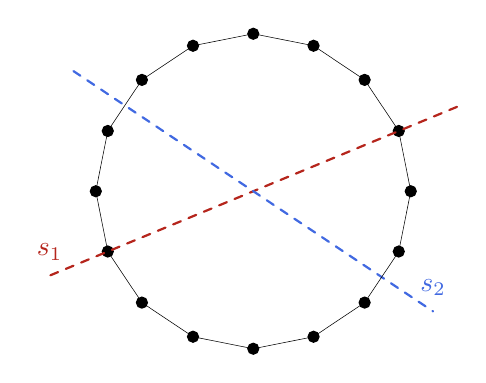
\begin{tikzpicture}[scale=2]
    \tkzInit
    \foreach \n/\a in
    {1/22.5,2/45,3/67.5,4/90,5/112.5,6/135,7/157.5,8/180,9/202.5,10/225,
    11/247.5,12/270,13/292.5,14/315,15/337.5,16/0} {%
     \tkzDefPoint(\a:1){\n}
    }
    \foreach \n in {1,2,...,16}{%
     \tkzDrawPoint[size=4,fill=black](\n)
    }
    \tkzDrawLine[thick,dashed,BrickRed](1,9)
    \tkzDefMidPoint(6,7)\tkzGetPoint{m1}
    \tkzDefMidPoint(14,15)\tkzGetPoint{m2}
    \tkzDrawLine[thick,dashed,RoyalBlue](m1,m2)
    \tkzLabelLine[pos=1.2,yshift=3mm](1,9){$\clr{s_1}$}
    \tkzLabelLine[pos=1.2,yshift=3mm](m1,m2){$\clb{s_2}$}
    \tkzDrawPolygon(1,2,3,4,5,6,7,8,9,10,11,12,13,14,15,16)
   \end{tikzpicture}
  \end{figure}
  \clearpage
  \part[10] Select those of the following four pairs of symmetries of the
  regular octagon (8 vertices) that \emph{\clr{generate all}} of its symmetries.
  \textbf{No explanation necessary}.
  \begin{figure}[H]
   \centering
   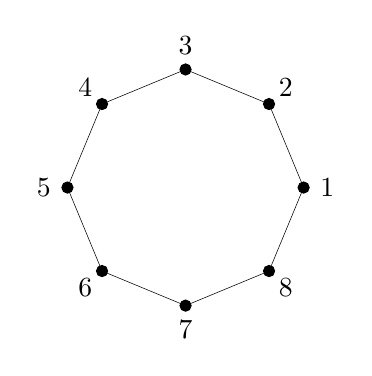
\begin{tikzpicture}[scale=1.5]
    \foreach \n/\a in {
     1/0,2/45,3/90,4/135,5/180,6/225,7/270,8/315
     } {
      \tkzDefPoint(\a:1){\n}
      \tkzDrawPoint[size=4,fill=black](\n)
      \node at (\a:1.2) {$\n$};
     }
     \tkzDrawPolygon(1,2,3,4,5,6,7,8)
   \end{tikzpicture}
   \caption*{Picture of the octagon for reference.}
  \end{figure}
  \begin{checkboxes}
   \item the rotation $\clr{r} =~\circlearrowleft 2 \cdot 360^{ \circ } / 8$ and
    the reflection $\clb{s}$ over the line passing through vertices $4$ and $8$,
   \item the rotation $\clr{r_1} = ~\circlearrowleft 3 \cdot 360^{ \circ } / 8$
    and the rotation $\clr{r_2} = ~\circlearrowleft 5 \cdot 360^{ \circ }$,
   \item the reflection $\clb{s_1}$ over the line passing through the midpoints
    of $23$ and $67$ and the reflection $\clb{s_2}$ over the line passing
    through the midpoints of $45$ and $18$,
   \item the rotation $\clr{r} =~\circlearrowleft 7 \cdot 360^{ \circ } / 8$
    and the reflection $\clb{s}$ over the line passing through vertices $3$ and
    $7$.
  \end{checkboxes}
  \part[10] Given reflections $\clr{s_1}$ and $\clb{s_2}$ of the heptagon (7
  vertices), compose them (and \emph{\clr{only}} them) to create the reflection
  $\clg{s_3}$ illustrated below. \textbf{Explain}.
  \begin{center}
   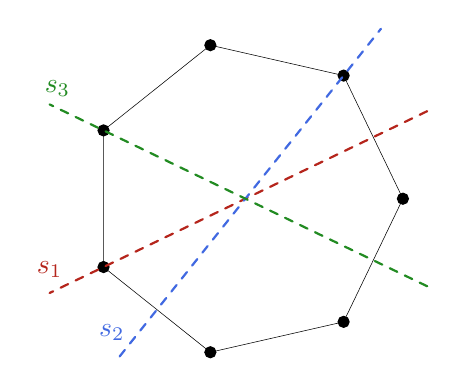
\begin{tikzpicture}[scale=2]
    \foreach \n/\a in {
     1/0.00,2/51.43,3/102.86,4/154.29,5/205.71,6/257.14,7/308.57
     } {
      \tkzDefPoint(\a:1){\n}
      \tkzDrawPoint[size=4,fill=black](\n)
     }
     \tkzDrawPolygon(1,2,3,4,5,6,7)
     \tkzDefMidPoint(1,2)\tkzGetPoint{m1}
     \tkzDefMidPoint(5,6)\tkzGetPoint{m2}
     \tkzDrawLine[thick,dashed,BrickRed](m1,5)
     \tkzDrawLine[thick,dashed,RoyalBlue](m2,2)
     \tkzLabelLine[pos=1.2,yshift=3mm](m1,5){$\clr{s_1}$}
     \tkzLabelLine[pos=-0.2,yshift=3mm,xshift=-1mm](m2,2){$\clb{s_2}$}

     \tkzDefMidPoint(1,7)\tkzGetPoint{m3}
     \tkzDrawLine[thick,dashed,ForestGreen](m3,4)
     \tkzLabelLine[pos=1.2,xshift=1mm,yshift=2mm](m3,4){$\clg{s_3}$}
   \end{tikzpicture}
  \end{center}
 \end{parts}
\end{questions}

\end{document}
